% NOTE - this is only a template without real arguments
\begin{entry}{Phase 1 completion}{Sep 2, 2021}
    \objective 
    
    Determine a data scheme for internal data (I.E. grid states and association data passed to the GO and logger.)
    Implement MCOutputLog
    Run a simulation and get output logs


    \outline

    \begin{itemize}
        \item Select data scheme (DICT OF DICTS)
        \item Add processing to EDMMeasurementProcessor
        \item Add accessor function to EDMMeasurementProcessor
        \item Write MCOutputLog
        \item Add accessor-logger routine to timekeeper
        \item Add log writing routine to timekeeper
        \item Add file closeout function to timekeeper closeout
        \item Test
        \item Add DER-EMs to model
        \item Add McInputInterface with a test function
        \item Add DERSHistoricalDataInput with a test function
        \item Test (Phase 1 closeout)

    \end{itemize}

    \procedures

    NOTE: I accidentially overwrote a bunch of information about previous steps, but it sums up to "it works". Info
    starts at "Add DER-EMs to model" for this sprint.


    \parameters
    
    N/A

    \observations

    Had a bunch of issues adding DER-EMs. A lot of them came from the fact that I was jumping back and forth between
    CIMHub and the Powergrid-Models repository. USE POWERGRID-MODELS FOR EVERYTHING. It grabs stuff from CIMHub, but the
    measurement stuff is in powergrid-models as well. A batch script could automate it, if written.

    Here is how the process works:

    \begin{enumerate}
        \item Create a text file containing the feeder ID and information about each DER. (See EGoT13\_der.txt in the
        powergrid-models/platform/DER folder.)
        \item Edit powergrid-models/platform/cimhubconfig.json to read "blazegraph\_url":
        "http://localhost:8889/bigdata/sparql".This was an issue for some reason.
        \item Edit powergrid-models/platform/DER/insert\_der.sh with the new filename. Run it. This will create a uuid
        file with IDs for the new DERs.
        \item Run the sparql query in the Data section below to verify DER-EMs have been added to the system.
        \item Edit/run powergrid-models/platform/list\_all\_measurements.sh
        \item Edit/run powergrid-models/platform/insert\_all\_measurements.sh
    \end{enumerate}

    I added three test DERs to the model at node 671. There were some initial struggles related to controlling them,
    but these all turned out to be due to incorrect mRIDs and typos. For results,
    see /Log Demos/testlog(9-17 binary input demo).csv. The DERs were set to 0 or 1kW, counting up in binary. The
    results were as expected once we knew what we were looking at: the measurement points all seem to be upstream of
    the inverter (and thus interconnected) and represent a single phase. So on each phase at node 671, we get 333W of
    power consumed per DER-EM that's "turned on". When all three are turned on, we get 1kW per phase, or 3kW total. This
    is as expected.

    Once I understood what I was looking at, the rest of the model came into focus. The only other dynamic load in the
    system is a house model that seems to be disconnected until the third (measurement) timestep. Those together with
    the DER-EMs had noticeable and consistent effects on current throughout the system. Apart from the house and its
    components, we have very basic energy consumers, compensators, and node to node line segment measurements, etc.



    I spent a long time trying to figure out the data scheme for the test input because I didn't understand that
    assignment is just a reference and I kept popping the "Time" data from an individual row in my input readout.
    Once I figured that out, the input manager and historical data DER-S worked pretty well. In this current state,
    the log columns need to be the mRIDs for the battery inverter control IDs (see query below.) Once per second,
    that message is ssent to the input handler which automatically changes the values for each mRID to the value in the
    cell. A single input command is sufficient for this (and will probably be sufficient from now on).

    Functional testing completed sat. There is an issue with the timecodes starting 6 seconds later than they should be,
    but this is minor at this point. I made a card to troubleshoot it later, it won't hold up progress.

    The following Test Plans were eligible for Phase 1 Testing:
    \begin{itemize}
        \item MC04
        \item MC05
        \item DER02
        \item DER07
        \item EDM08
        \item EDM10
    \end{itemize}


    \data
    
    \begin{verbatim}
        # Storage - DistStorage
        PREFIX r:  <http://www.w3.org/1999/02/22-rdf-syntax-ns#>
        PREFIX c:  <http://iec.ch/TC57/CIM100#>
        SELECT ?name ?bus ?ratedS ?ratedU ?ipu ?ratedE ?storedE ?state ?p ?q ?id ?fdrid (group_concat(distinct ?phs;separator="\n") as ?phases) WHERE {
         ?s r:type c:BatteryUnit.
         ?s c:IdentifiedObject.name ?name.
         ?pec c:PowerElectronicsConnection.PowerElectronicsUnit ?s.
        # feeder selection options - if all commented out, query matches all feeders
        #VALUES ?fdrid {"_C1C3E687-6FFD-C753-582B-632A27E28507"}  # 123 bus
        VALUES ?fdrid {"_49AD8E07-3BF9-A4E2-CB8F-C3722F837B62"}  # 13 bus
        #VALUES ?fdrid {"_5B816B93-7A5F-B64C-8460-47C17D6E4B0F"}  # 13 bus assets
        #VALUES ?fdrid {"_4F76A5F9-271D-9EB8-5E31-AA362D86F2C3"}  # 8500 node
        #VALUES ?fdrid {"_67AB291F-DCCD-31B7-B499-338206B9828F"}  # J1
        #VALUES ?fdrid {"_9CE150A8-8CC5-A0F9-B67E-BBD8C79D3095"}  # R2 12.47 3
         ?pec c:Equipment.EquipmentContainer ?fdr.
         ?fdr c:IdentifiedObject.mRID ?fdrid.
         ?pec c:PowerElectronicsConnection.ratedS ?ratedS.
         ?pec c:PowerElectronicsConnection.ratedU ?ratedU.
         ?pec c:PowerElectronicsConnection.maxIFault ?ipu.
         ?s c:BatteryUnit.ratedE ?ratedE.
         ?s c:BatteryUnit.storedE ?storedE.
         ?s c:BatteryUnit.batteryState ?stateraw.
           bind(strafter(str(?stateraw),"BatteryState.") as ?state)
         ?pec c:PowerElectronicsConnection.p ?p.
         ?pec c:PowerElectronicsConnection.q ?q.
         OPTIONAL {?pecp c:PowerElectronicsConnectionPhase.PowerElectronicsConnection ?pec.
         ?pecp c:PowerElectronicsConnectionPhase.phase ?phsraw.
           bind(strafter(str(?phsraw),"SinglePhaseKind.") as ?phs) }
         bind(strafter(str(?s),"#_") as ?id).
         ?t c:Terminal.ConductingEquipment ?pec.
         ?t c:Terminal.ConnectivityNode ?cn.
         ?cn c:IdentifiedObject.name ?bus
        }
        GROUP by ?name ?bus ?ratedS ?ratedU ?ipu ?ratedE ?storedE ?state ?p ?q ?id ?fdrid
        ORDER by ?name
    \end{verbatim}

    \results
    
    All tests completed sat. Phase 1 of the ME is now complete.


\end{entry}


%\begin{entry}{CMake Error running EGOT-DCM Dockerfile}{Dec 02, 2020}
%    \objective
%
%    Determine the cause of the CMake error while running the dockerfile and modify file to get it to successfully build.
%
%    \outline
%
%    \begin{itemize}
%        \item Try running to see if it was just Lorry or a machine issue.
%        \item If it is a machine issue, modify configurations to ensure interoperability.
%        \item If I get the error track down its cause and modify dockerfile to fix.
%        \item Repeat until all builds are successful.
%    \end{itemize}
%
%    \procedures
%
%    \begin{itemize}
%        \item \mint{console}|git clone https://github.com/EGoT-DCS-SunSpec-Modbus|
%        \item \mint{console}|docker build -f Dockerfile.buster -t egot-dcs .|
%        \item \mint{console}|docker container run -i egot-dcs|
%    \end{itemize}
%
%    \observations
%
%    \begin{error}{Cmake Error: No CMAKE\_CXX\_COMPILER found}
%        \begin{figure}[H]
%            \centering
%            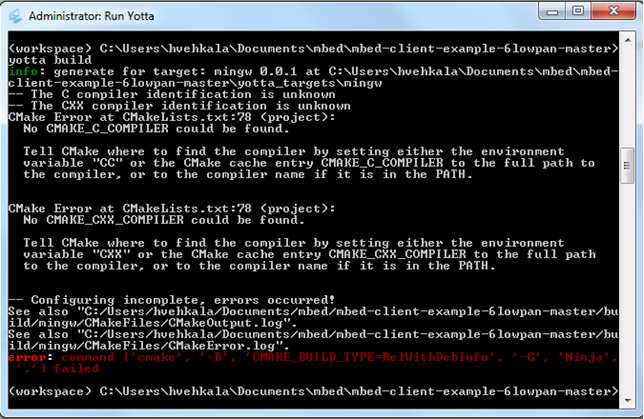
\includegraphics[height=4in]{Fall2020/Figures/cmake_error.png}
%        \end{figure}
%
%        Solution: what you need to do found at \cite{CMAKE-Forum}
%    \end{error}
%
%    \results
%
%    Short: No.
%
%    Long: Well...
%
%
%\end{entry}